\documentclass[11pt]{article}
\usepackage{subfigure,wrapfig,graphicx,booktabs,fancyhdr,amsmath,amsfonts,appendix,tikz}
\usepackage{bm,amssymb,amsthm,wasysym,color,fullpage,setspace,multirow,placeins}
\usepackage{pgfplots}
\pgfplotsset{compat=1.18}
\usepackage{amsmath,amssymb}
\usepackage{tcolorbox}

% Custom math commands
\newcommand{\vb}{\boldsymbol}
\newcommand{\vbh}[1]{\hat{\boldsymbol{#1}}}
\newcommand{\vbb}[1]{\bar{\boldsymbol{#1}}}
\newcommand{\vbt}[1]{\tilde{\boldsymbol{#1}}}
\newcommand{\vbs}[1]{{\boldsymbol{#1}}^*}
\newcommand{\vbd}[1]{\dot{{\boldsymbol{#1}}}}
\newcommand{\vbdd}[1]{\ddot{{\boldsymbol{#1}}}}
\newcommand{\by}{\times}
\newcommand{\tr}{{\rm tr}}
\newcommand{\cpe}[1]{\left[{#1} \times\right]}
\newcommand{\sfrac}[2]{\textstyle\frac{#1}{#2}}

% Title and Author Information
\title{Advanced Scientific Engineering \\ Homework 4}
\author{Jacob Hands}
\date{October 18, 2024}

\begin{document}
\maketitle


\section{QR Factorization of Matrix \(A\)}

Given matrix \( A \):

\[
A = \begin{bmatrix} 
3 & 0 \\
0 & 2 \\
1 & 0
\end{bmatrix}
\]

We want to perform the QR factorization \( A = QR \), where:
- \( Q \) is an orthogonal matrix.
- \( R \) is an upper triangular matrix.

Step 1: Construct the orthonormal set (columns of \(Q\))

1. First, take the first column of \( A \), \( \mathbf{a_1} = \begin{bmatrix} 3 \\ 0 \\ 1 \end{bmatrix} \), and normalize it:
   \[
   \|\mathbf{a_1}\| = \sqrt{3^2 + 0^2 + 1^2} = \sqrt{10}
   \]
   So, the first column of \(Q\) is:
   \[
   \mathbf{q_1} = \frac{1}{\sqrt{10}} \begin{bmatrix} 3 \\ 0 \\ 1 \end{bmatrix} = \begin{bmatrix} \frac{3}{\sqrt{10}} \\ 0 \\ \frac{1}{\sqrt{10}} \end{bmatrix}
   \]

2. For the second column, take \( \mathbf{a_2} = \begin{bmatrix} 0 \\ 2 \\ 0 \end{bmatrix} \), and normalize it:
   \[
   \|\mathbf{a_2}\| = \sqrt{0^2 + 2^2 + 0^2} = 2
   \]
   So, the second column of \( Q \) is:
   \[
   \mathbf{q_2} = \frac{1}{2} \begin{bmatrix} 0 \\ 2 \\ 0 \end{bmatrix} = \begin{bmatrix} 0 \\ 1 \\ 0 \end{bmatrix}
   \]

Thus, the matrix \( Q \) is:
\[
Q = \begin{bmatrix}
\frac{3}{\sqrt{10}} & 0 \\
0 & 1 \\
\frac{1}{\sqrt{10}} & 0
\end{bmatrix}
\]

Step 2: Compute \(R\)

Using the relation \( R = Q^T A \), we calculate \( R \):

\[
Q^T = \begin{bmatrix}
\frac{3}{\sqrt{10}} & 0 & \frac{1}{\sqrt{10}} \\
0 & 1 & 0
\end{bmatrix}
\]

Now, multiply \( Q^T \) by \( A \):
\[
R = Q^T A = \begin{bmatrix}
\frac{3}{\sqrt{10}} & 0 & \frac{1}{\sqrt{10}} \\
0 & 1 & 0
\end{bmatrix} \begin{bmatrix}
3 & 0 \\
0 & 2 \\
1 & 0
\end{bmatrix}
\]

Carrying out the matrix multiplication:
\[
R = \begin{bmatrix}
\frac{3}{\sqrt{10}} \cdot 3 + \frac{1}{\sqrt{10}} \cdot 1 & 0 \\
0 \cdot 3 + 1 \cdot 2 & 2
\end{bmatrix}
= \begin{bmatrix}
\frac{9}{\sqrt{10}} + \frac{1}{\sqrt{10}} & 0 \\
0 & 2
\end{bmatrix}
= \begin{bmatrix}
\sqrt{10} & 0 \\
0 & 2
\end{bmatrix}
\]

Thus, \( R = \begin{bmatrix}
\sqrt{10} & 0 \\
0 & 2
\end{bmatrix} \).

Final QR Factorization

\[
\boxed{A = QR = 
\begin{bmatrix}
\frac{3}{\sqrt{10}} & 0 \\
0 & 1 \\
\frac{1}{\sqrt{10}} & 0
\end{bmatrix} \begin{bmatrix}
\sqrt{10} & 0 \\
0 & 2
\end{bmatrix}
}
\]

% \begin{figure}[!ht]
%     \centering
%     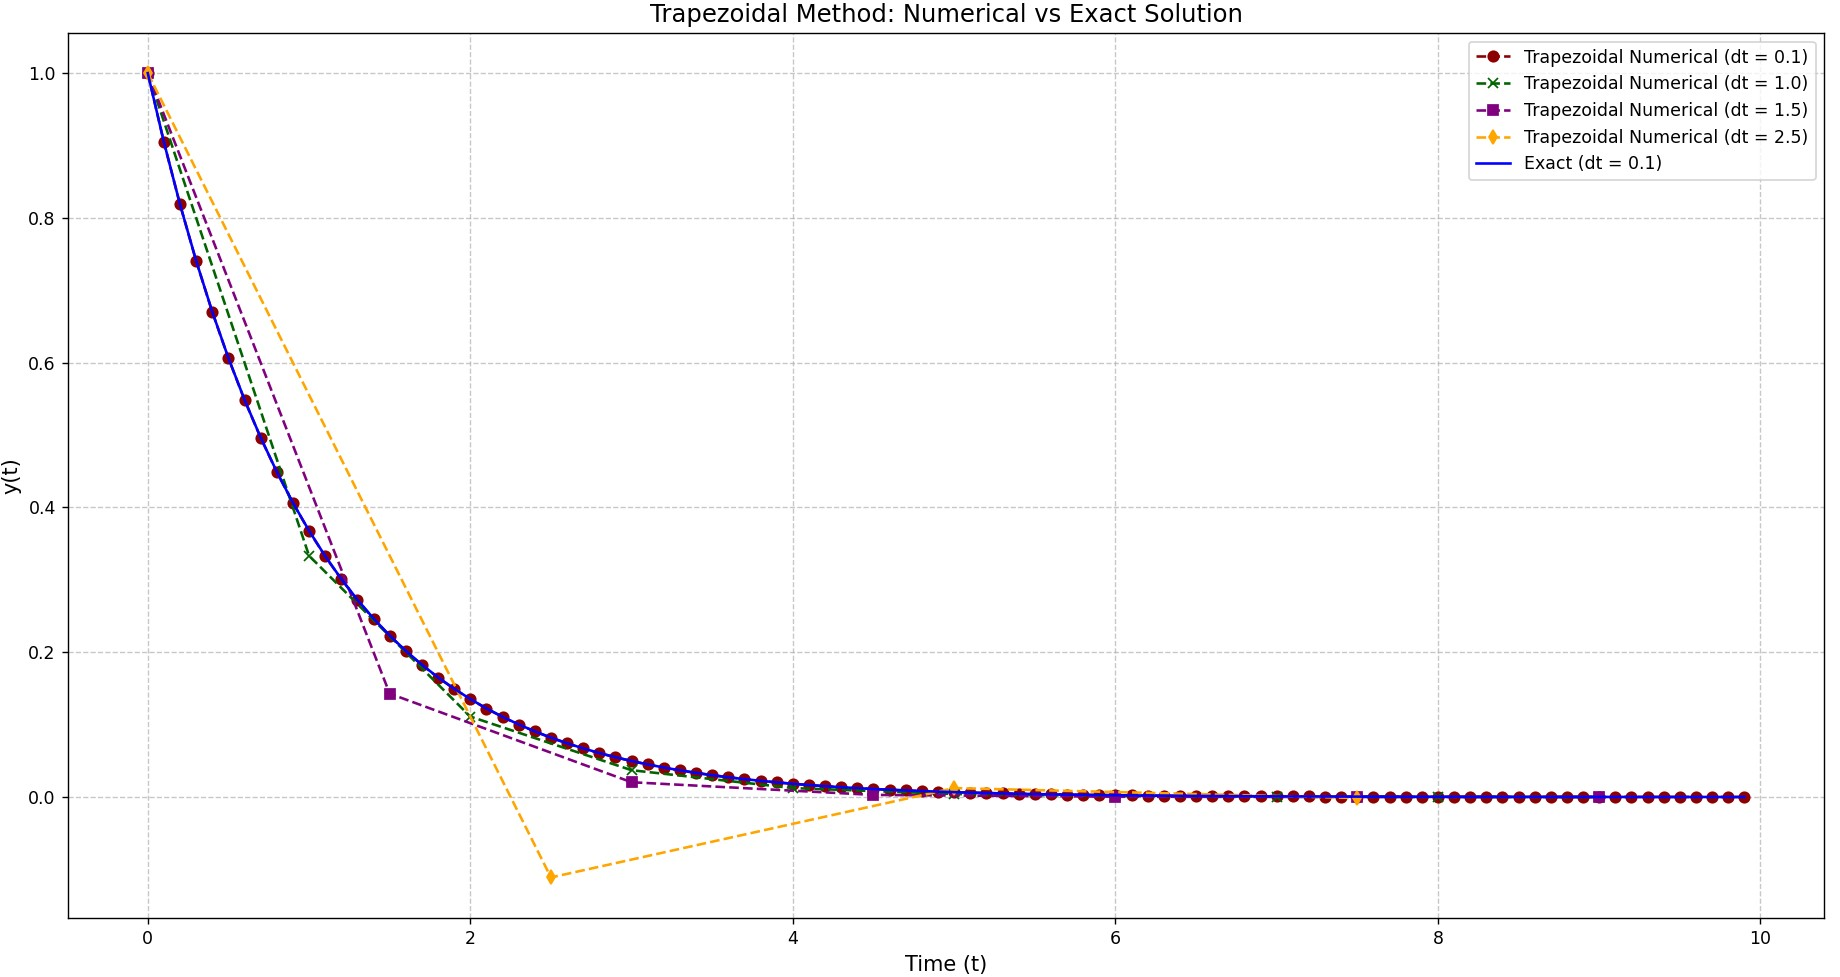
\includegraphics[width= 1 \textwidth]{images/Trapezoidal method.jpg}
%     \caption{Trapezoidal Method Numerical vs Exact Solution}
%     \label{fig:1}
%   \end{figure}
%   \FloatBarrier


\section{Weighted Least Squares for Closest Line}

By hand, find the closest line in a weighted least squares sense that approximates the following data points: 
\[
(0,0), (1,2), (2,1), (3,6)
\]
with point weights:
\[
2/10, 3/10, 3/10, 2/10.
\]
Hint: The inverse of a 2x2 matrix is as follows:
\[
\begin{bmatrix} 
a & b \\ 
c & d 
\end{bmatrix}^{-1} = \frac{1}{ad-bc} 
\begin{bmatrix} 
d & -b \\ 
-c & a 
\end{bmatrix}
\]

We begin by defining the system:
\[
A = 
\begin{bmatrix}
1 & 0 \\
1 & 1 \\
1 & 2 \\
1 & 3
\end{bmatrix}, \quad
\hat{\mathbf{u}} = 
\begin{bmatrix}
a \\
b
\end{bmatrix}, \quad
\hat{\mathbf{b}} = 
\begin{bmatrix}
0 \\
2 \\
1 \\
6
\end{bmatrix}
\]

The transpose of matrix $A$ is:
\[
A^T = 
\begin{bmatrix}
1 & 1 & 1 & 1 \\
0 & 1 & 2 & 3
\end{bmatrix}
\]

The weight matrix is:
\[
C = \text{diag}\left(\frac{1}{\sigma_n^2}\right)
\]

Using the weighted least squares formula:
\[
\hat{\mathbf{u}}^* = (A^T C A)^{-1} A^T C \hat{\mathbf{b}}
\]

Substituting the values:
\[
\hat{\mathbf{u}}^* = 
\left( 
\begin{bmatrix} 
1 & 1 & 1 & 1 \\ 
0 & 1 & 2 & 3 
\end{bmatrix}
\begin{bmatrix}
\frac{1}{.2^2} & 0 & 0 & 0 \\
0 & \frac{1}{.3^2} & 0 & 0 \\
0 & 0 & \frac{1}{.3^2} & 0 \\
0 & 0 & 0 & \frac{1}{.2^2}
\end{bmatrix}
\begin{bmatrix} 
1 & 0 \\
1 & 1 \\
1 & 2 \\
1 & 3 
\end{bmatrix}
\right)^{-1}
\begin{bmatrix} 
1 & 1 & 1 & 1 \\ 
0 & 1 & 2 & 3 
\end{bmatrix}
\begin{bmatrix}
\frac{1}{.2^2} & 0 & 0 & 0 \\
0 & \frac{1}{.3^2} & 0 & 0 \\
0 & 0 & \frac{1}{.3^2} & 0 \\
0 & 0 & 0 & \frac{1}{.2^2}
\end{bmatrix}
\begin{bmatrix}
0 \\
2 \\
1 \\
6
\end{bmatrix}
\]

After solving this system, we obtain:
\[
\begin{bmatrix}
a \\
b
\end{bmatrix} =
\begin{bmatrix}
-0.24977 \\
1.85882
\end{bmatrix}
\]

Thus, the equation of the line is:
\[\boxed{
y = -0.24977x + 1.85882}
\]

\begin{figure}[!ht]
  \centering
  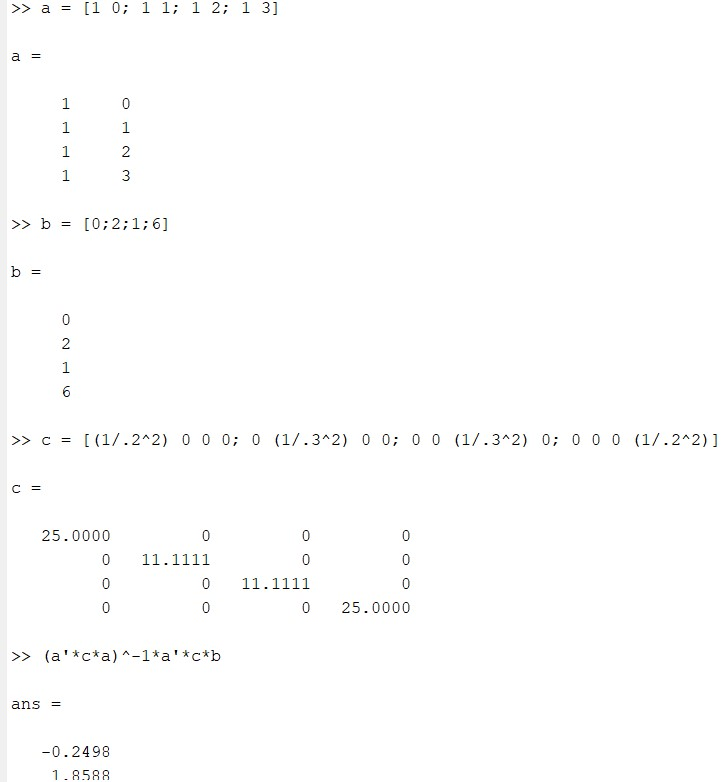
\includegraphics[width= 1 \textwidth]{images/prob2.jpg}
  \caption{MatLab Code For Solution}
  \label{fig:1}
\end{figure}
\FloatBarrier

\section{Deriving the Growth Term \( G \) for the Heat Equation}

Given the heat equation:
\[
u_t = D u_{xx}
\]
where \( D \) is the diffusion coefficient, we are asked to use the backward Euler method for the time derivative and centered differences for the spatial derivative.

### Step 1: Centered Difference Approximation
The centered difference approximation for the second spatial derivative \( u_{xx} \) is:
\[
u_{xx}(x) = \frac{u(x+h) - 2u(x) + u(x-h)}{h^2}
\]

### Step 2: Backward Euler Method
The backward Euler approximation for the time derivative is:
\[
u^{n+1} = u^n + \Delta t \cdot f(u^{n+1}, u^n)
\]
which simplifies to:
\[
\frac{u^{n+1} - u^n}{\Delta t} = D \frac{u^{n+1}(x+h) - 2u^{n+1}(x) + u^{n+1}(x-h)}{h^2}
\]

### Step 3: Substituting \( u = G e^{ikx} \)
We now substitute \( u = G e^{ikx} \) into the equation for both the time and spatial derivatives:
\[
\frac{G e^{ikx} - e^{ikx}}{\Delta t} = D \frac{e^{ik(x+h)} - 2 e^{ikx} + e^{ik(x-h)}}{h^2}
\]
Using the identity:
\[
e^{ik\Delta x} + e^{-ik\Delta x} = 2 \cos(k\Delta x)
\]
the equation becomes:
\[
\frac{G - 1}{\Delta t} = D \frac{2 (\cos(k\Delta x) - 1)}{h^2}
\]

### Step 4: Solving for \( G \)
Rearranging the equation to solve for \( G \):
\[
G - 1 = D \cdot \frac{2 (\cos(k\Delta x) - 1)}{h^2} \cdot \Delta t
\]
\[
G = 1 + \frac{2D(\cos(k\Delta x) - 1)}{h^2} \cdot \Delta t
\]

Thus, the growth factor \( G \) is:
\[
\boxed{G = \frac{2D (\cos(k \Delta x) - 1)}{\Delta t} + 1}
\]
\section{Analysis of the Function \( f(x) = 4 + 8x^2 - x^4 \)}

### 1. Find the first and second derivatives of \( f(x) \)

We are given the function:
\[
f(x) = 4 + 8x^2 - x^4
\]

The first derivative \( f'(x) \) is:
\[
f'(x) = \frac{d}{dx}(4 + 8x^2 - x^4) = 16x - 4x^3
\]

The second derivative \( f''(x) \) is:
\[
f''(x) = \frac{d}{dx}(16x - 4x^3) = 16 - 12x^2
\]

### 2. Find the y-intercept and determine any maxima or minima

The y-intercept occurs when \( x = 0 \):
\[
f(0) = 4 + 8(0)^2 - (0)^4 = 4
\]
Thus, the y-intercept is at \( (0, 4) \).

To find the critical points, set \( f'(x) = 0 \):
\[
16x - 4x^3 = 0
\]
\[
4x(4 - x^2) = 0
\]
\[
x = 0, \quad x = \pm 2
\]

Now check the second derivative at these points:
- At \( x = 0 \):
  \[
  f''(0) = 16 > 0 \quad \Rightarrow \quad \text{local minimum at } (0, 4)
  \]
- At \( x = \pm 2 \):
  \[
  f''(2) = f''(-2) = 16 - 12(2)^2 = -32 < 0 \quad \Rightarrow \quad \text{local maximum at } (2, 20) \text{ and } (-2, 20)
  \]

### 3. Sketch the Graph and Determine Symmetry

\begin{center}
    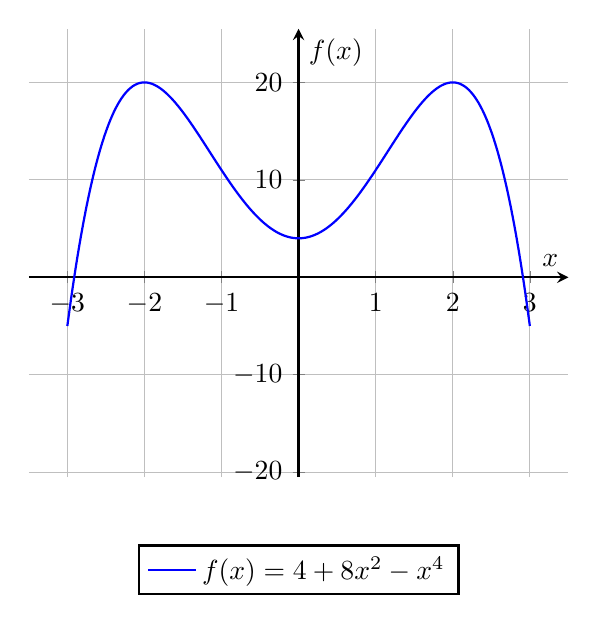
\begin{tikzpicture}
        \begin{axis}[
            domain=-3:3, % Set the x range
            samples=100, % Number of samples for smooth curve
            axis lines=middle, % Place the axes at the middle
            xlabel=$x$, % Label for x-axis
            ylabel=$f(x)$, % Label for y-axis
            xtick={-3,-2,-1,0,1,2,3}, % Set x-axis ticks
            ytick={-20,-10,0,10,20}, % Set y-axis ticks
            ymin=-20, ymax=25, % Set y range
            xmin=-3, xmax=3, % Set x range
            grid=both, % Add grid
            thick, % Line thickness
            enlargelimits={abs=0.5}, % Enlarge limits slightly
            legend style={at={(0.5,-0.15)}, anchor=north, legend columns=-1}, % Position legend
        ]
        \addplot[
            domain=-3:3,
            samples=100,
            smooth,
            thick,
            blue,
        ]{4 + 8*x^2 - x^4};
        \addlegendentry{$f(x) = 4 + 8x^2 - x^4$}
        \end{axis}
    \end{tikzpicture}
    \end{center}
% \begin{figure}[!ht]
%     \centering
%     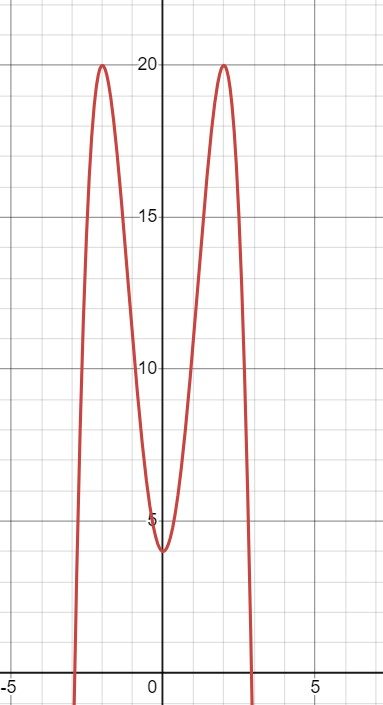
\includegraphics[width= 1 \textwidth]{images/sketch3.jpg}
%     \caption{Sketch of the Graph}
%     \label{fig:1}
%   \end{figure}
%   \FloatBarrier

Since \( f(x) \) only involves even powers of \( x \), it is symmetric about the y-axis, indicating that the function is even.

### 4. Use Newton's Method to Approximate the x-intercept near \( x = 3 \)

We apply Newton's method with the following iteration formula:
\[
x_{n+1} = x_n - \frac{f(x_n)}{f'(x_n)}
\]
Using the code provided:

\begin{verbatim}
// Function f(x) = 4 + 8x^2 - x^4
func f(x float64) float64 {
    return 4 + 8*x*x - math.Pow(x, 4)
}

// First derivative f'(x) = 16x - 4x^3
func f_prime(x float64) float64 {
    return 16*x - 4*math.Pow(x, 3)
}

// Newton's method for finding x-intercept
func newtonsMethod(x0 float64, iterations int) float64 {
    x := x0
    for i := 0; i < iterations; i++ {
        x = x - f(x)/f_prime(x)
        fmt.Printf("Iteration %d: x = %.6f\n", i+1, x)
    }
    return x
}

func main() {

    // Part 4: Newton's Method for x-intercept near x = 3
    fmt.Println("\nNewton's method to find x-intercept near x = 3:")
    initialGuess := 3.0
    iterations := 2
    xIntercept := newtonsMethod(initialGuess, iterations)
    fmt.Printf("Approximate x-intercept: %.6f\n", xIntercept)
}
\end{verbatim}

The output after two iterations approximates the x-intercept as:
\[
x \approx 2.910723
\]

Thus, the approximate \( x \)-intercept near \( x = 3 \) is \( 2.910723 \).

\begin{figure}[!ht]
    \centering
    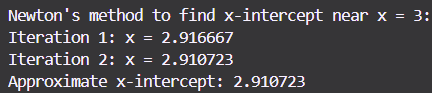
\includegraphics[width= 1 \textwidth]{images/x_1.png}
    \label{fig:1}
  \end{figure}
  \FloatBarrier

\section{Analysis of the Function \( f(x) = x^3 - 3x - 3 \)}

### 1. Find all extrema and points of inflection

Given the function \( f(x) = x^3 - 3x - 3 \), we first compute the first and second derivatives:

\[
f'(x) = 3x^2 - 3
\]
\[
f''(x) = 6x
\]

To find the critical points, set \( f'(x) = 0 \):

\[
3x^2 - 3 = 0 \quad \Rightarrow \quad x^2 = 1 \quad \Rightarrow \quad x = \pm 1
\]

Now, calculate the function values at these critical points:
\[
f(1) = (1)^3 - 3(1) - 3 = -5
\]
\[
f(-1) = (-1)^3 - 3(-1) - 3 = -1
\]

Now, check the second derivative at these points to determine whether they are maxima or minima:
- At \( x = 1 \):
  \[
  f''(1) = 6(1) = 6 > 0 \quad \Rightarrow \quad \text{absolute minimum at } (1, -5)
  \]
- At \( x = -1 \):
  \[
  f''(-1) = 6(-1) = -6 < 0 \quad \Rightarrow \quad \text{absolute maximum at } (-1, -1)
  \]

### 2. Is the function odd, even, or neither?

To check if the function is odd, we test the property \( f(-x) = -f(x) \). For \( x = 1 \):
\[
f(1) = -5, \quad f(-1) = -1
\]
Since \( f(-1) \neq -f(1) \), the function is not odd.

To check if the function is even, we would test for symmetry across the y-axis, but there is no symmetry. Therefore, the function is neither odd nor even.

### 3. Sketch of the function \( f(x) = x^3 - 3x - 3 \)

\begin{center}
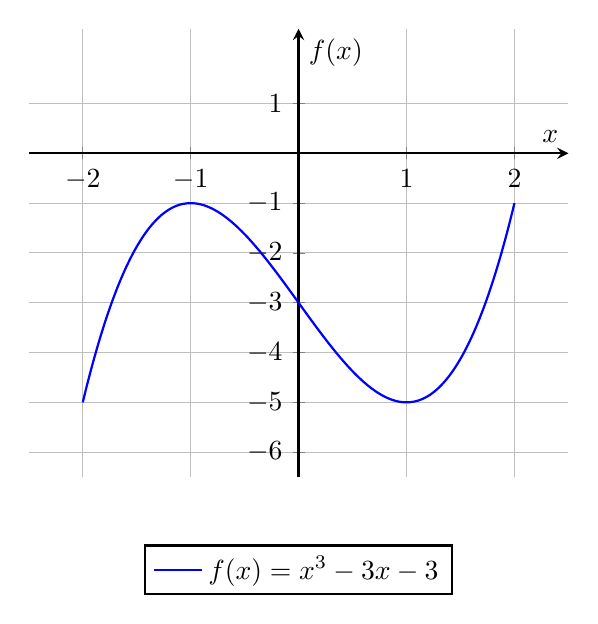
\begin{tikzpicture}
    \begin{axis}[
        domain=-2:2, % Set the x range
        samples=100, % Number of samples for smooth curve
        axis lines=middle, % Place the axes at the middle
        xlabel=$x$, % Label for x-axis
        ylabel=$f(x)$, % Label for y-axis
        xtick={-2,-1,0,1,2}, % Set x-axis ticks
        ytick={-6,-5,-4,-3,-2,-1,0,1}, % Set y-axis ticks
        ymin=-6, ymax=2, % Set y range
        xmin=-2, xmax=2, % Set x range
        grid=both, % Add grid
        thick, % Line thickness
        enlargelimits={abs=0.5}, % Enlarge limits slightly
        legend style={at={(0.5,-0.15)}, anchor=north, legend columns=-1}, % Position legend
    ]
    \addplot[
        domain=-2:2,
        samples=100,
        smooth,
        thick,
        blue,
    ]{x^3 - 3*x - 3};
    \addlegendentry{$f(x) = x^3 - 3x - 3$}
    \end{axis}
\end{tikzpicture}
\end{center}

### 4. Newton's Method for Approximating the \( x \)-Intercept

We apply Newton's method to approximate the x-intercept near \( x_0 = 2 \), using the formula:
\[
x_{n+1} = x_n - \frac{f(x_n)}{f'(x_n)}
\]

The function and its derivative are:
\[
f(x) = x^3 - 3x - 3, \quad f'(x) = 3x^2 - 3
\]

Using an initial guess \( x_0 = 2 \) and performing two iterations:

\begin{verbatim}
// Function f(x) = x^3 - 3x - 3
func f(x float64) float64 {
    return math.Pow(x, 3) - 3*x - 3
}

// First derivative f'(x) = 3x^2 - 3
func f_prime(x float64) float64 {
    return 3*math.Pow(x, 2) - 3
}

// Newton's method for finding x-intercept
func newtonsMethod(x0 float64, iterations int) float64 {
    x := x0
    for i := 0; i < iterations; i++ {
        x = x - f(x)/f_prime(x)
        fmt.Printf("Iteration %d: x = %.6f\n", i+1, x)
    }
    return x
}

func main() {
    // Part 4: Newton's Method for x-intercept near x = 2
    initialGuess := 2.0
    iterations := 2
    xIntercept := newtonsMethod(initialGuess, iterations)
    fmt.Printf("Approximate x-intercept: %.6f\n", xIntercept)
}
\end{verbatim}

The output after two iterations is approximately:
\[
x \approx 2.103836
\]

Thus, the approximate x-intercept is \( x \approx 2.103836 \).

\begin{figure}[!ht]
    \centering
    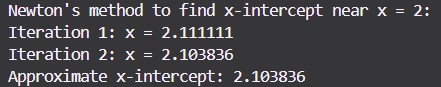
\includegraphics[width= 1 \textwidth]{images/prob_5.jpg}
    \label{fig:1}
  \end{figure}
  \FloatBarrier

  \section{Go Code for Bisection Method}

Below is the Go code that calculates the root using the Bisection Method for \( f(x) = x^2 - 3 = 0 \) in the interval \( [1, 2] \).

\begin{verbatim}
package main

import (
	"fmt"
	"math"
)

// Function f(x) = x^2 - 3 = 0
func f(x float64) float64 {
	return math.Pow(x, 2) - 3
}

func main() {
	// Initialize variables as float64
	var lower_bound float64 = 1
	var upper_bound float64 = 2
	var root float64
	var iteration_count int
	var tolerance float64 = 0.000001 // Tolerance to check how close the result is to zero

	// Set up the bisection method
	for {
		middle := (lower_bound + upper_bound) / 2
		potential_root := f(middle)

		// checks the root tolerance
		if math.Abs(potential_root) <= tolerance {
			root = middle
			break
		}

		// Adjust the bounds
		if potential_root > 0 {
			upper_bound = middle
		} else {
			lower_bound = middle
		}
		// Keep count of the iterations
		iteration_count++
	}

	// Output the result
	fmt.Printf("The calculated root is: %.6f\n", root)
	fmt.Printf("The number of iterations it took: %d\n", iteration_count)
}
\end{verbatim}

  The approximate solution using the bisection method is:
\[
x \approx 1.732051
\]

The amount of iterations taken:
\[
n = 19
\]

  \begin{figure}[!ht]
    \centering
    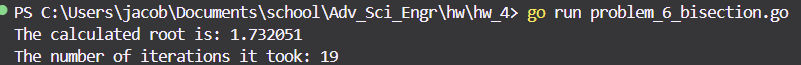
\includegraphics[width= 1 \textwidth]{images/x_3.png}
    \label{fig:1}
  \end{figure}
  \FloatBarrier

\end{document}
